% !TEX root = ../thesis.tex
% [H] means put the figure HERE, directly when you input this code.
% Remove this to let LaTeX place the figure where it decides is best


\begin{figure}[H]
	\centering
	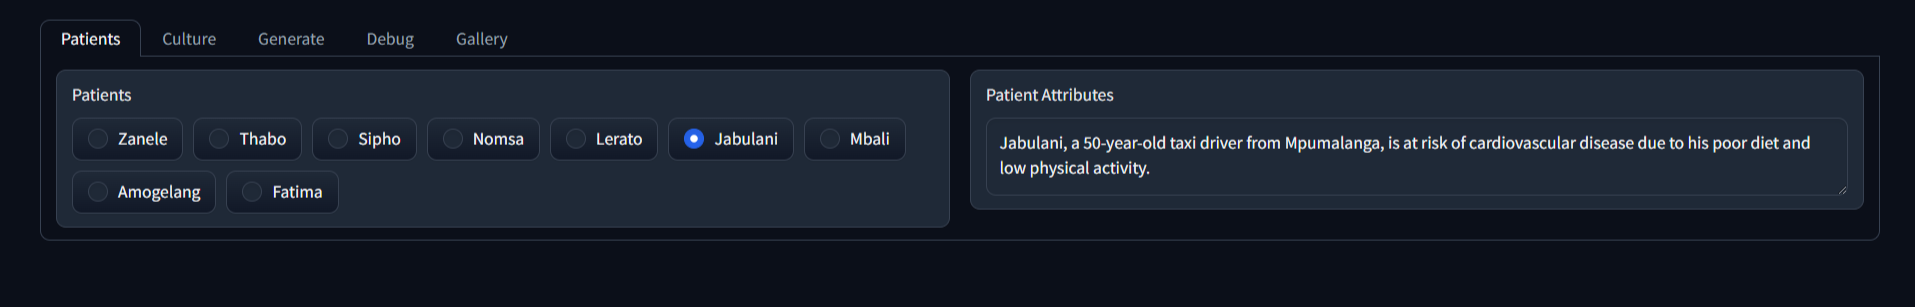
\includegraphics[width=1.0\textwidth]{./graphics/t1.png}
	\caption[System design image pending.]{
Select a patient and their details are loaded and displayed.
	\label{fig:system_design}
	}
\end{figure}

\begin{figure}[H]
	\centering
	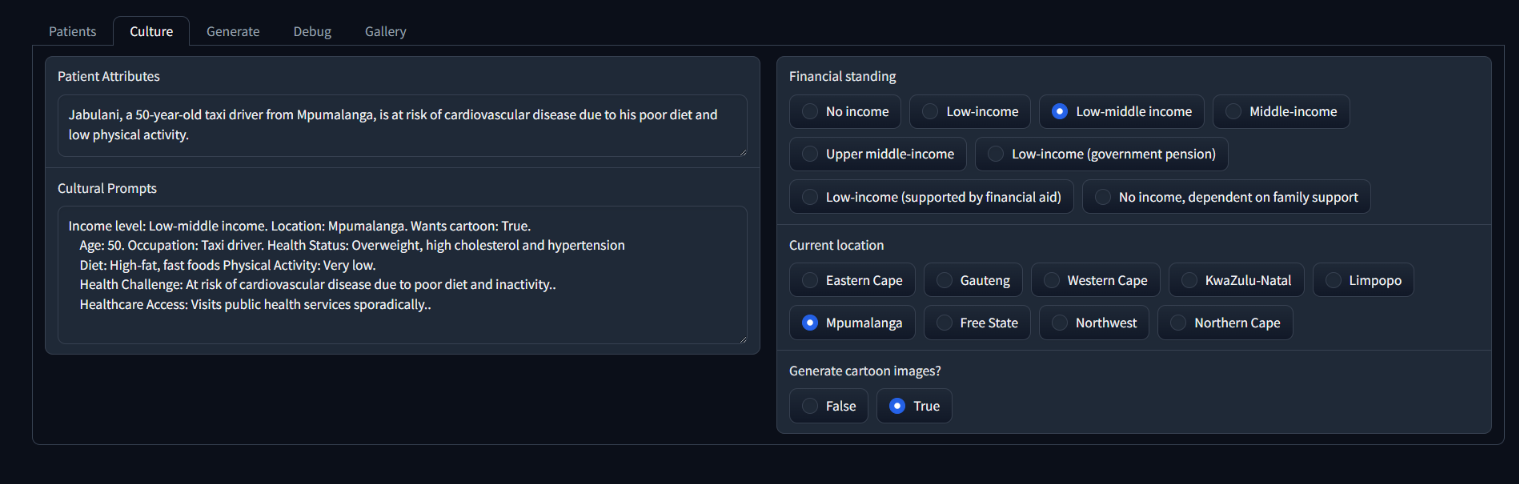
\includegraphics[width=1.0\textwidth]{./graphics/t2.png}
	\caption[System design image pending.]{
On the Culture tab, select culture details and image style.
	\label{fig:system_design}
	}
\end{figure}

\begin{figure}[H]
	\centering
	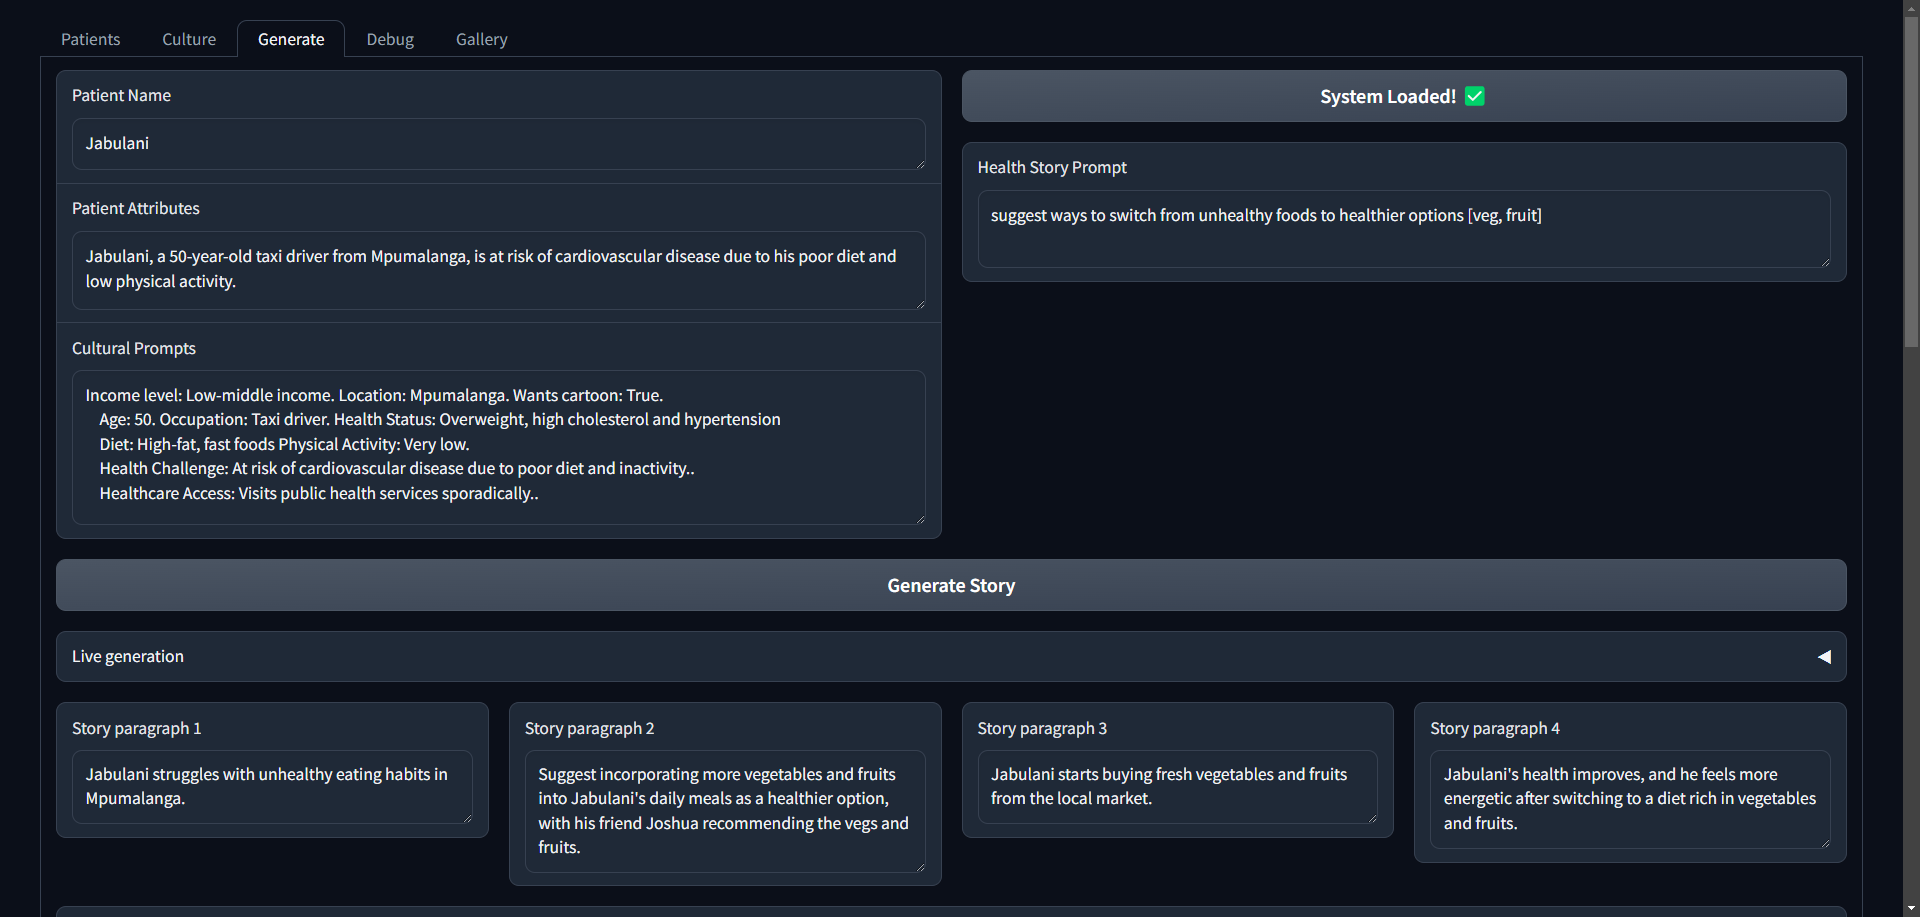
\includegraphics[width=1.0\textwidth]{./graphics/t3.png}
	\caption[System design image pending.]{
On the Generate tab, fill in the Health Story prompt and generate a story with its prompts.
	\label{fig:system_design}
	}
\end{figure}

\begin{figure}[H]
	\centering
	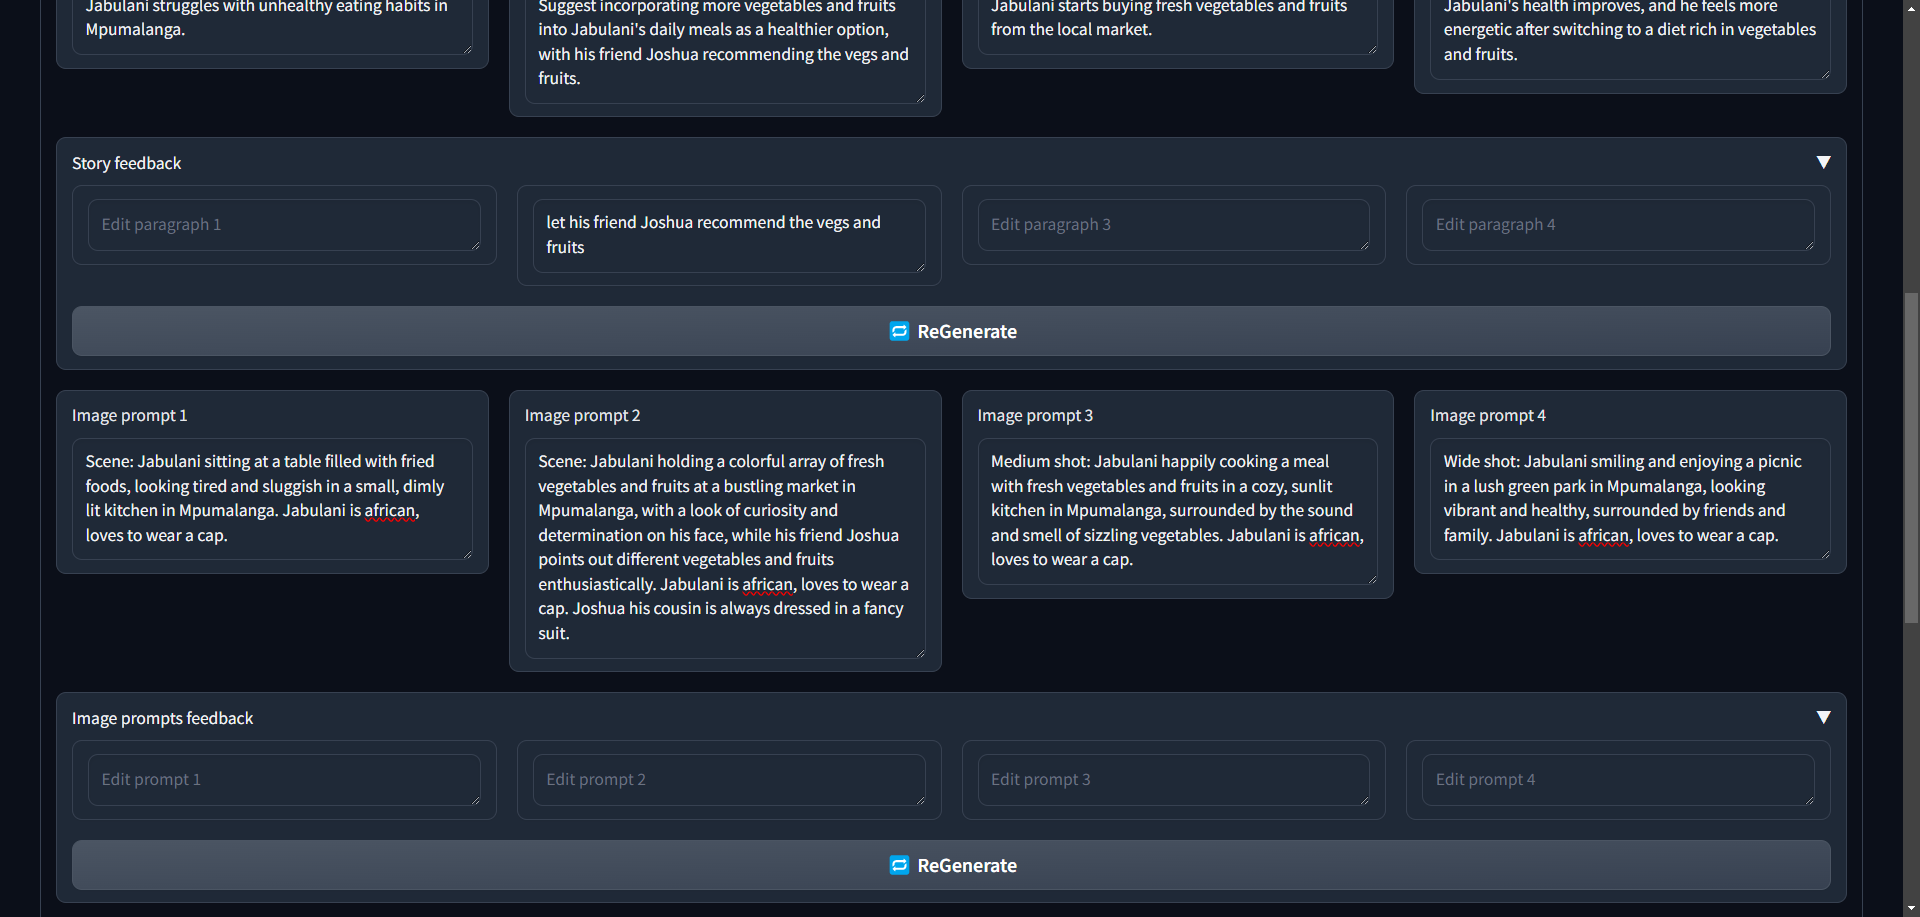
\includegraphics[width=1.0\textwidth]{./graphics/t4.png}
	\caption[System design image pending.]{
Feedback on story paragraphs is used by the system to refine the story.
	\label{fig:system_design}
	}
\end{figure}

\begin{figure}[H]
	\centering
	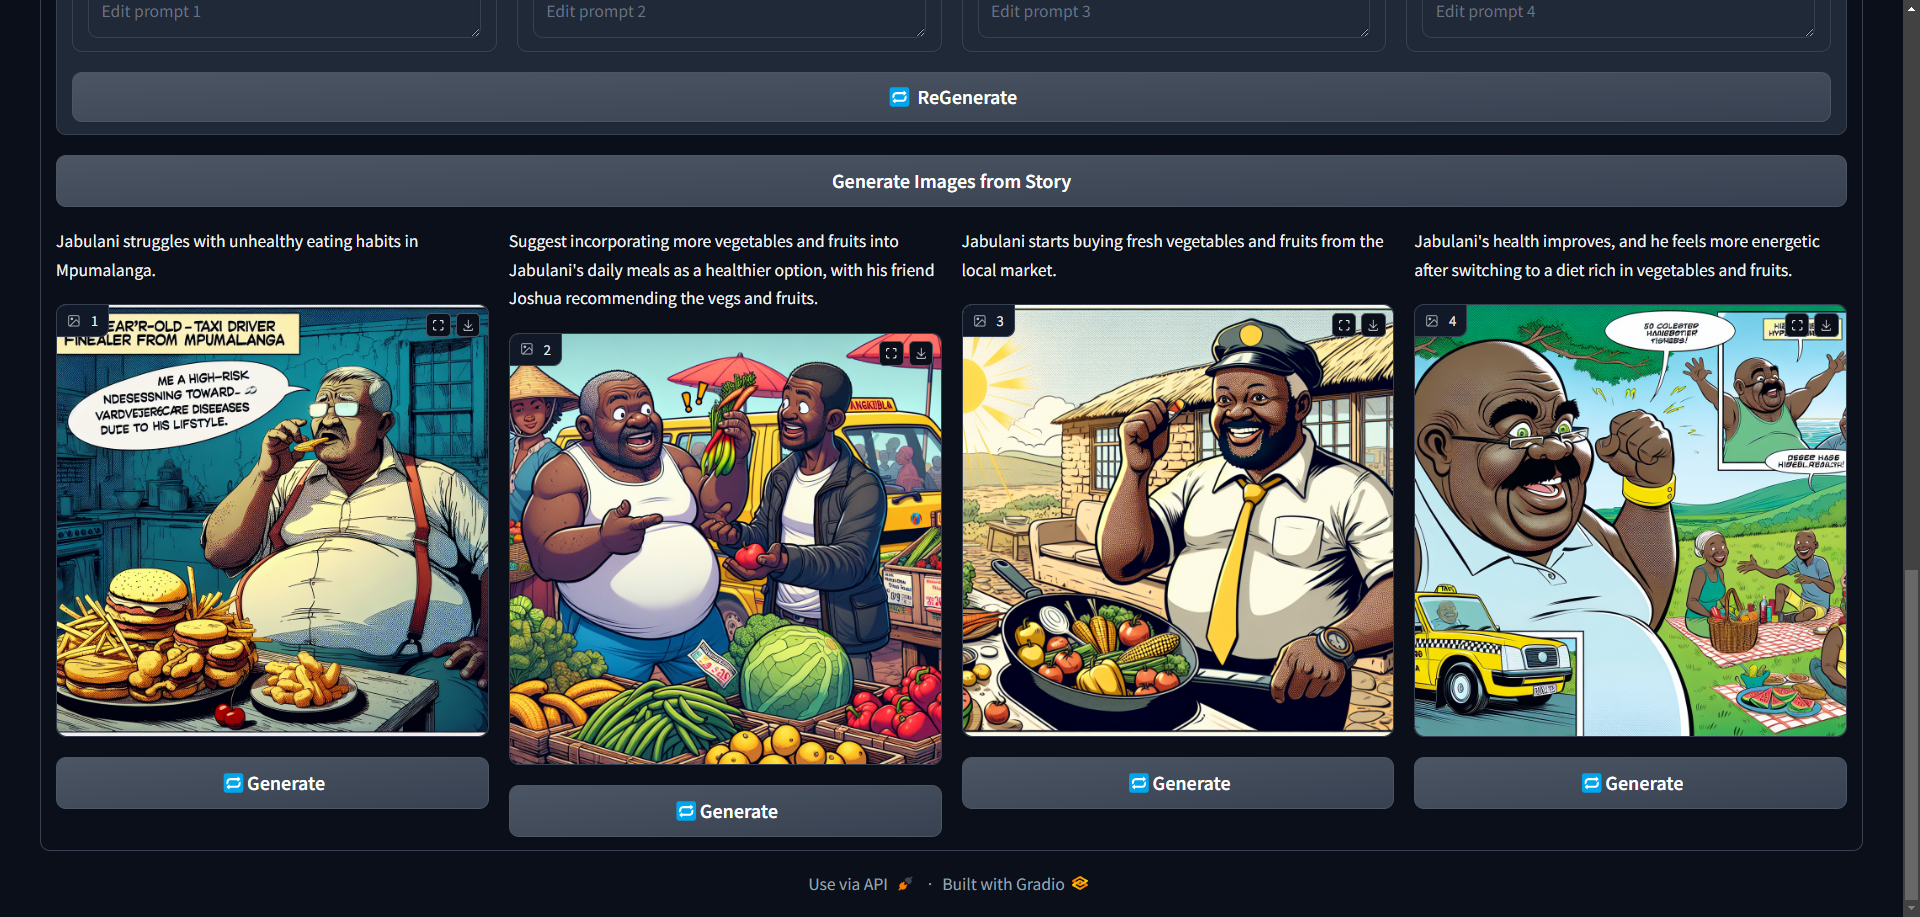
\includegraphics[width=1.0\textwidth]{./graphics/t5.png}
	\caption[System design image pending.]{
Generate the accompanying images when you're happy with the story.
	\label{fig:system_design}
	}
\end{figure}